\section{Lösungsidee}
\subsection{Kreismittelpunkterkennung}
Um möglichst effizient Kreismittelpunkte zu bestimmen, mache ich mir zunächst folgende Eigenschaft von Kreisen zunutze: Am Mittelpunkt eines Kreises ist der Abstand zu der äußeren Umrandung des Kreises in jede Richtung gleich. Dieser Abstand entspricht dem Radius.

In einem Bild lassen sich solche Punkte finden, indem man von jedem schwarzen Bildpunkt misst, wie weit man sich auf dem Bild in vertikale wie horizontale Richtung "`bewegen"' kann, ohne auf ein weißes Feld zu stoßen. Wenn dieser Abstand nach rechts, links, oben und unten gleich groß ist, genügt der Punkt der erstgenannten Eigenschaft von Kreisen. 

Von einem Vergleich des Abstandes in weitere Richtungen (wie z.B. in diagonale Richtung) sollte man bei einer Bitmap aus Pixeln absehen, da bei einer Bitmap aus quadratischen Pixeln diagonale Messungen oder gar Messungen unter beliebigem Winkel ungenaue Ergebnisse liefern. 
Zwar sind solche Messungen prinzipiell möglich, liefern aber anders als vertikale oder horizontale Messungen keine ganzzahligen Ergebnisse, da eine Pixeldiagonale \(\sqrt{2}\) Pixelseiten lang ist.
\footnote{: \( \vert \begin{pmatrix}1\\1\end{pmatrix} \vert = \sqrt{2}\)}

\begin{figure}[!ht]
	\centering	
	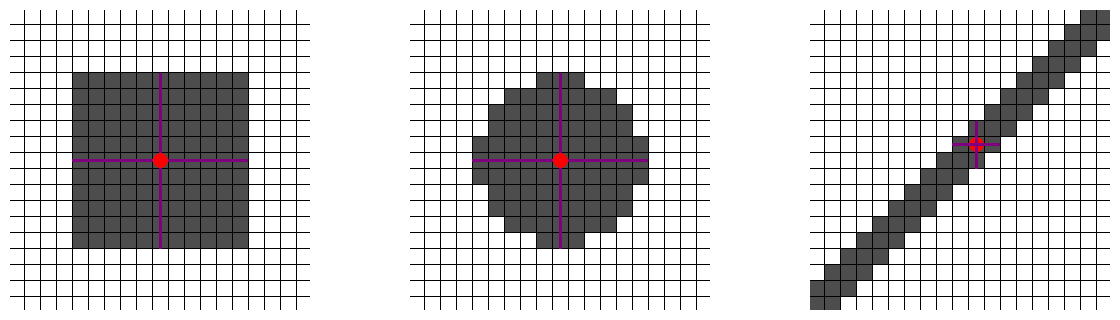
\includegraphics[width=0.8\textwidth]{Grafiken/durchmesservergleich}
	\caption{Versch. Formen mit eingezeichnetem Mittelpunkt (erstes Kriterium)}
	\label{abb:mischformen}
\end{figure}

Da die erstgenannte Eigenschaft jedoch auch auf Punkte in Quadraten und anderen unregelmäßigen Formen zutrifft (s. Grafik \ref{abb:mischformen}), muss für eine zuverlässige Erkennung eine zweite Eigenschaft von Kreisen genutzt werden: Bei bekanntem Durchmesser kann die Fläche eines Kreises mit der Kreisformel\footnote{: \(\frac{\pi d^2}{4}\)} bestimmt werden.
Diese Soll-Fläche kann anschließend mit der tatsächlichen Fläche des vermeintlichen Kreises verglichen werden. Sollte das Delta zwischen diesen beiden Flächengrößen nahe 0 sein, handelt es sich mit sehr großer Wahrscheinlichkeit um einen Kreismittelpunkt. 
Dass Soll und Ist identisch sind ist unmöglich, da sich ein Kreis in einer Bitmap aus quadratischen Pixeln zusammensetzt. Ein Kreis lässt sich nicht aus Quadraten exakt zusammensetzen.

Da die Wahrscheinlichkeit eines False Positives nach Überprüfen beider Kriterien sehr gering ist, nehme ich an, dass jeder Punkt, auf den beide Kriterien zutreffen, ein Kreismittelpunkt ist. 
Allerdings ist es aufgrund von Kompressionsartefakten oder einer geringen Bildauflösung möglich, dass es mehrere sehr nahe liegende Punkte gibt, auf die diese Bedingungen zutreffen. Damit der Mittelpunkt für jeden Kreis eindeutig bestimmt wird, merkt sich der Algorithmus bei der Flächenermittlung die Felder, von denen bereits die Fläche ermittelt wurde. 
So kann der Algorithmus bei Pixeln, die schon beachtet wurden, abbrechen. Schließlich wurde entweder schon ein Mittelpunkt gefunden oder es hat sich herausgestellt, dass es sich nicht um einen Kreis handelt.

\begin{wrapfigure}{r}{0.35\textwidth}
  \centering
  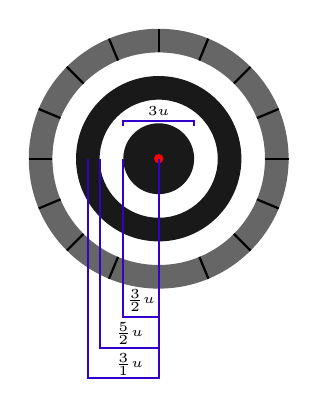
\begin{tikzpicture}[scale=0.3]
\fill[black!90!white] (0,0) circle [radius=1.5];
\fill[black!90!white, even odd rule] (0,0) circle[radius=2.5] circle[radius=3.5];
\fill[black!60!white, even odd rule] (0,0) circle[radius=4.5] circle[radius=5.5];

\foreach \angle in {0, 22.5, 45, 67.590, 90, 112.5, 135, 157.5, 180, 202.5, 225, 247.5, 270, 292.5, 315, 337.5} 
	\draw[thick] (\angle:4.5) -- (\angle:5.5);

\fill[red] (0,0) circle[radius=0.2];

\draw[color=blue!60!violet, thick] (-1.5,1.4) -- ++(0, 0.2) -- ++(1.5, 0) +(0, 0.4)node[black]{\tiny{\(3u\)}}+(0, 0) -- ++(1.5, 0) -- ++(0, -0.2);

\draw[color=blue!60!violet, thick] (0,0) -- (0,-6.7) -- +(-1.5, 0) -- (-1.5,0);
\draw[color=blue!60!violet, thick] (0,0) -- (0,-8) -- +(-2.5, 0) -- (-2.5,0);
\draw[color=blue!60!violet, thick] (0,0) -- (0,-9.3) -- +(-3, 0) -- (-3,0);

\draw (-0.75, -6) node{\tiny{\(\frac{3}{2}u\)}};
\draw (-1.25, -7.4) node{\tiny{\(\frac{5}{2}u\)}};
\draw (-1.25, -8.7) node{\tiny{\(\frac{3}{1}u\)}};
\end{tikzpicture}
  \caption{Größenverhältnisse}
  \label{abb:dims}
\end{wrapfigure}

\subsection{Kreisringerkennung}
Danach gilt es noch zu bestimmen, ob es sich bei dem Kreis um einen Mittelpunkt eines \task{}s handelt, schließlich sollen Mittelpunkte sonstiger Kreise nicht ausgegeben werden. Dies wäre nicht im Sinne der nachfolgenden Teilaufgaben. Hierzu können wir uns die Proportionen eines \task{}s zu nutze machen:

Der Durchmesser des Kreises ist als \(3u\) definiert, der Kreisring und die Zwischenräume haben eine Breite von \(1u\). 
Daraus folgt, dass wenn man den Kreismittelpunkt in eine beliebige Richtung um den Kreisdurchmesser (\(3u\)) verschiebt, der neue Punkt im mittleren, durchgehend schwarzen, Kreisring liegen muss. (siehe Abb. \ref{abb:dims})

Von diesem Punkt ausgehend können wir wieder den Ist-Flächeninhalt des Kreisringes mit dem erwarteten Flächeninhalt vergleichen. Da der Kreisring aus einem Kreis mit einem Durchmesser von \(7u\), von dem die inneren \(5u\) ausgeschnitten wurden, besteht, muss der Kreisring folgenden Flächeninhalt haben:\footnote{\url{https://de.wikipedia.org/wiki/Kreisring}}

\begin{equation}
	A=\frac{\pi{}\times(D^2-d^2)}{4}=\frac{\pi{}\times((7u)^2-(5u)^2)}{4}=6\pi{}u^2
\end{equation}

Die Wahrscheinlichkeit eines Erkennungsfehlers ist nach Überprüfung des Radius und den beiden Flächenvergleichen sehr gering. Im Beispielbild, dass ich um einen Kreis ohne Mittelring ergänzt habe, liegt die Erkennungsrate bei 100\%.

\section{Umsetzung}
Zunächst implementierte ich mithilfe von ImageIO, einer Klasse der Java-Standardbibliothek, eine Bildeinleseprozedur. Da ImageIO nur RGB-JP(E)Gs, PNGs, BMPs und GIFs einlesen kann, habe ich zusätzlich einen Wrapper für ImageMagick\footnote{\url{http://www.imagemagick.org/}, GPLv3-kompatible freie Lizenz. Enthalten in den Repositories der gängigen Linux-Distributionen, Binarys für weitere Betriebssysteme auf der Entwicklerseite.} geschrieben. 
Wenn dieser über die entsprechende Checkbox in der GUI zugeschaltet wird, können alle gängigen Bildformate gelesen werden. 
Nachteil ist eine deutlich längere Einlesezeit. Darüber hinaus muss ImageMagick lokal installiert sein und der Befehl \texttt{convert} im PATH enthalten sein.\footnote{Getestet unter Arch, Ubuntu und Fedora. Nicht unter sonstigen Betriebssystemen wie z.B. Windows getestet.} 

Darauf überlegte ich mir eine möglichst effiziente Datenstruktur für Grafiken, da die Interaktion über ImageIO mit Bitmaps nicht sonderlich effizient ist. Da für die Erkennung von Kreisen in einer Grafik genaue Informationen über die Farbe eines Bildpunktes nicht relevant sind, kann das Bild beim Einlesevorgang in ein boolesches 2D-Array überführt werden: In diesem Array, das die gleiche Größe wie das eingelesene Bild besitzt, sind schwarze Bildpunkte als True gespeichert. In der in Teilaufgabe 1 gegebenen Schwarz-Weiß-Grafik ist die Bestimmung schwarzer Bildbunkte noch simpel: Schwarze Bildpunkte sind im Array True, sonstige sind false.
Nach der Einleseprozedur ist ein Binärbild gegeben.

\subsection{Kreismittelpunkterkennung}
Um in diesem Binärbild die Punkte zu bestimmen, deren Abstand zum äußeren Rand eines True-Segmentes sich in alle vier Richtungen gleichen, bestimme ich zunächst die Länge von aufeinanderfolgenden Streifen aus als True markierten Feldern. In seperaten Arrays für horizontale und vertikale Streifen speichere ich für jeden Pixel seine gesamte Streifenlänge.
Alle Felder, die vorher als False markiert wurden, haben eine Streifenlänge von 0. 

Die erste Eigenschaft aus der Aufgabenstellung lässt sich mit der soeben vorberechneten Information nun so umsetzen, dass nach aufeinander liegenden Mittelpunkten gleich langer vertikaler und horizontaler Streifen gesucht wird.
An solchen Stellen ist die erste Eigenschaft gegeben, da in alle Richtungen der Abstand zum Rand des True-Segmentes identisch ist. Wie in der Lösungsidee dargestellt, entspricht dann eine Streifenlänge dem Kreisdurchmesser.

Für diese Suche bestimme ich zunächst alle Mittelpunkte horizontaler Streifen. Dies geschieht, indem ich mit einer linearen Suche über das ganze Bild alle Koordinaten bestimme, deren horizontale Streifenlänge größer null ist und denen ein False-Pixel vorrausgeht.
Hiermit finde ich Anfangsstellen horizontaler Streifen. Ich habe definiert, dass Streifen sich nicht über mehrere Zeilen erstrecken können, sodass es für jeden Streifen in einer Zeile einen Anfangspunkt gibt.
Wenn auf die x-Koordinate dieser Anfangsstelle die Hälfte der Länge des Streifens hinzuaddiert wird, erhalte ich den Mittelpunktes des Streifens.
Die y-Koordinate ist für eine \textit{horizontale} Komponente durchgehend gleich und ist daher aus der Schleife der linearen Suche gegeben.

An dem soeben bestimmten Mittelpunkten lese ich die Längen der vertikalen Streifen an der gleichen Stelle aus. Wenn die Differenz zwischen diesen beiden Längen 0 oder 1 ist, werte ich die Längen der Komponenten als gleich.
Ein Fehler von 1 kann durch Ungenauigkeiten bei ganzzahliger Division leicht entstehen und ist daher an dieser Stelle unwesentlich.

Anschließend überprüfe ich, ob an dieser Stelle auch der vertikale Streifen seinen Mittelpunkt hat. Nur dann ist der Abstand an dieser Stelle in alle Richtungen identisch. Dazu verschiebe ich den Mittelpunkt um eine halbe vertikale Komponentenlänge - 1 (halber Durchmesser = Radius) nach oben und unten. Da dieser Wert kleiner als der Kreisradius ist, müssen beide Punkte noch innerhalb des Kreises liegen und damit True sein. Außerdem muss die Streifenlänge an allen Stellen identisch sein.
Eine Überprüfung über die gesamte Komponentenlänge wäre ebenfalls möglich, würde aber gerade bei hochaufgelösten Bildern unnötig Zeit verbrauchen. Aufgrund des Vergleiches der Komponentenlängen ist ein False Positive unwahrscheinlich.

Für den Vergleich der Ist- und Soll-Fläche wird zunächst die Soll-Fläche mit der Kreisformel berechnet. Der Durchmesser des Kreises ist mit der Länge einer der beiden Zusammenhängigkeitskomponenten gegeben. Die tatsächliche Größe der Fläche kann mit einer Flood-Fill\footnote{\url{https://en.wikipedia.org/wiki/Flood_fill}} ermittelt werden.
Die Flood-Fill-Methode wird mit dem Mittelpunkt aufgerufen und erhöht einen Zähler. Die Methode ruft sich anschließend für alle angrenzenden True-Felder selbst auf. Um zu verhindern, dass die Rekursion unendlich stattfindet, wird für jedes Feld, dass von der "`Flut"' berührt wurde, in einem weiteren Array eine ID gespeichert.
Diese ID wird fortlaufend für jeden Flood-Fill-Durchlauf vergeben. Im Code der Flood-Fill ist der Rekursion die Bedingung vorangestellt, dass nur Felder, für die noch keine ID vergeben wurde, aufgerufen werden. Damit entspricht nach Ablauf der Flood-Fill der Zählerinhalt der Ist-Fläche.

Da aufgrund der oftmals verlustbehafteten Kompression und Ungenauigkeiten bei der Abbildung eines Kreises mit quadratischen Pixeln das Ist niemals exakt dem Soll entspricht, akzeptiert das Programm eine Abweichung von bis zu 10\%. 

\subsection{Kreisringerkennung}
Schließlich muss noch das Vorhandensein des Kreisringes wie in der Lösungsidee beschrieben verifiziert werden. Die Implementierung erfolgte wie auch beim Flächenvergleich über eine Flood-Fill, allerdings wurde entsprechend die andere Formel für das Soll verwendet. Außerdem wird bei diesem Vergleich eine Abweichung von bis zu 30\% akzeptiert, da aufgrund der kleineren Fläche des Ringes kleine absolute Abweichungen einem größeren Prozentsatz entsprechen.

\pagebreak
\section{Beispiele}
Die erkannten Kreismittelpunkte sind mit violetten Fadenkreuzen markiert. Das Beispielbild der Aufgabenstellung habe ich um einen Kreis ohne umschließenden Ring ergänzt. Dieser wird korrekterweise nicht markiert. Außerdem habe ich einen weiteren Testfall mit Kreisen wechselnder Größe und einer störenden Grafik erstellt.
\begin{figure}[!ht]
	\centering	
	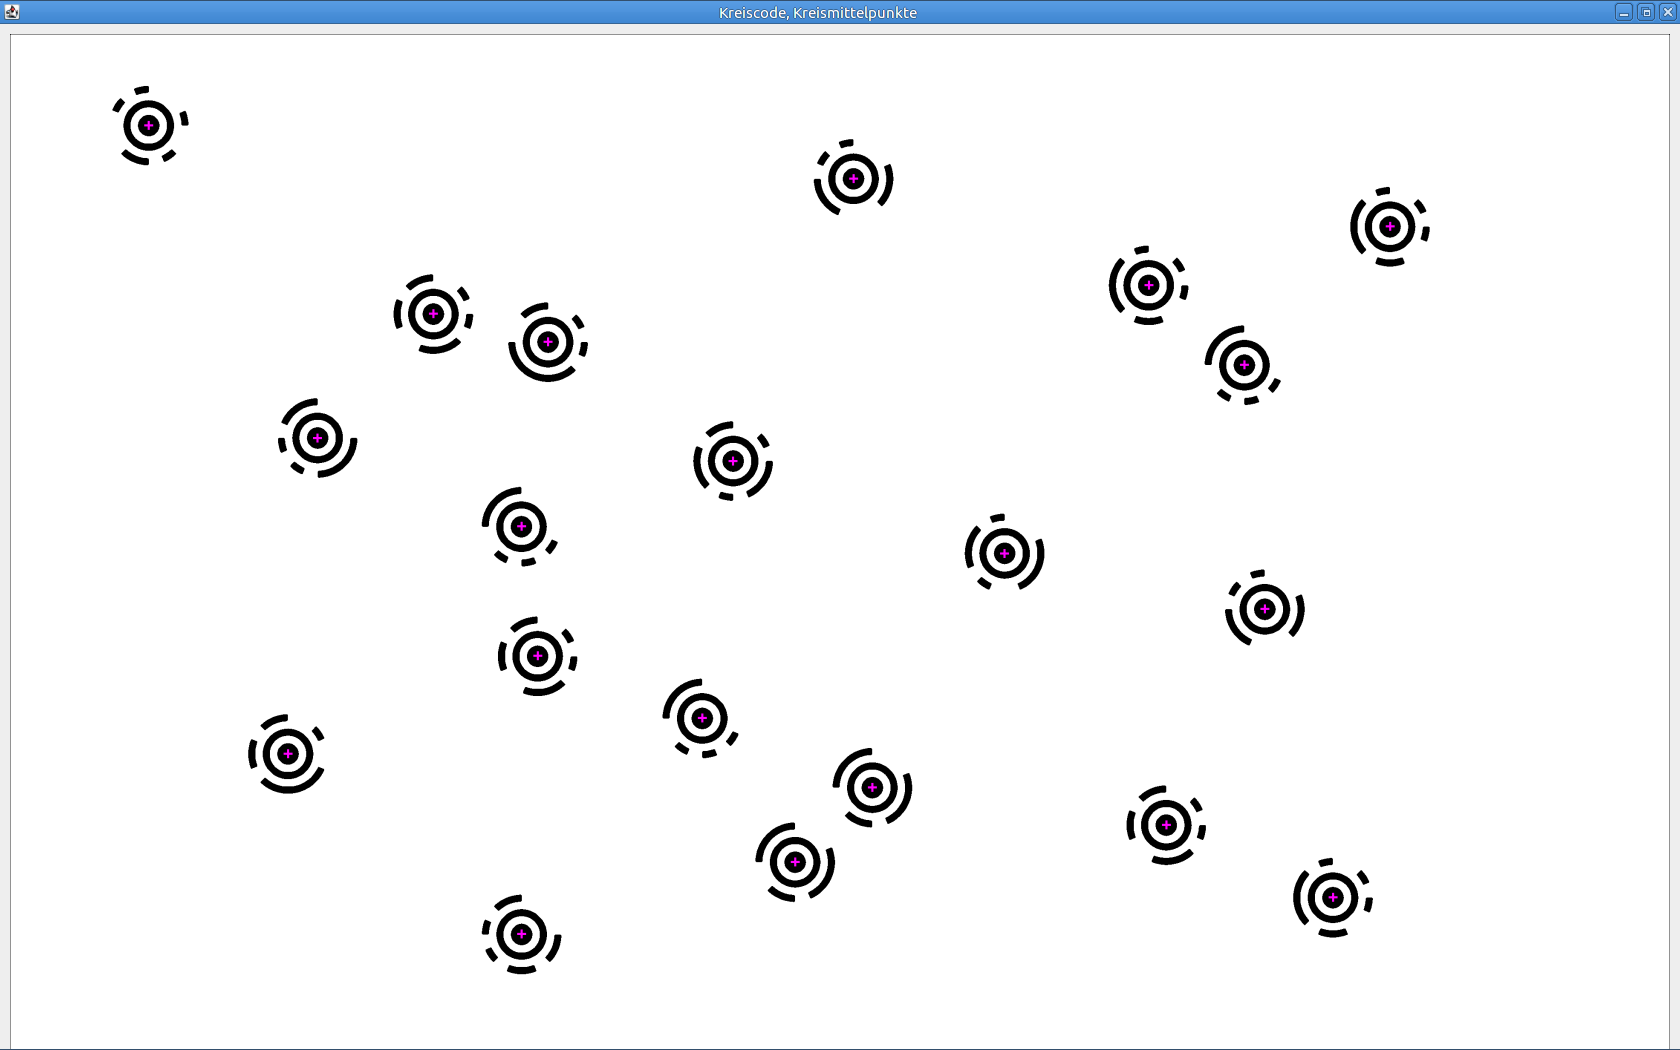
\includegraphics[width=0.7\textwidth]{Grafiken/sek1bsp1}
	\caption{Erweitertes Beispielbild aus der Aufgabenstellung}
\end{figure}
\vfill{}
\begin{figure}[!ht]
	\centering	
	\includegraphics[width=0.7\textwidth]{Grafiken/sek1bsp2}
	\caption{Zweiter Testfall}
\end{figure}
